\section{Exercices}

\begin{exocor}[Orage et boussole] 
On cherche dans cet exercice à déterminer le
champ magnétique créé par un éclair lors d'un orage.  En première
approximation, un éclair peut-être assimilé à un fil rectiligne de rayon
$a = \unit{10}{\centi \meter}$ parcouru par un courant d'intensité constante
$I = \unit{10^5}{\ampere}$.  
\begin{enumerate} 
	\item Faire un schéma modélisant un éclair. 
	Quel est le repère adapté au problème ici ?  
	\item  
	De quelle(s) variable(s) dépend l'amplitude du champ magnétique ? 
	Par quel vecteur est-il porté ?  
	Dessiner les lignes du champ magnétique produit par cet éclair.
	\item Déterminer l'expression du champ magnétique créé par l'éclair.
	      Vérifier l'homogénéité de votre expression.  
	\item L'aiguille d'une boussole peut se retrouver désaimantée 
	lorsqu'elle est placée dans un champ supérieur à 
	$B_L = \unit{2 \times 10^{-3}}{\tesla}$. À quelle distance minimale d'un
	éclair doit donc se trouver une boussole pour ne pas être désaimantée ?
\end{enumerate} 
\end{exocor}

\begin{exocor}[Bobines de Helmholtz]
Les bobines de Helmholtz sont un dispositif expérimental constitué de 
deux bobines circulaires de même rayon, parallèles et placées à une distance
égale à leur rayon. Dans cet exercice, on cherche à déterminer le champ magnétique
généré par ce système.

On considère tout d'abord une spire de rayon $R$, d'axe $Oz$, 
parcouru par un courant $I$ et
placée en $z = 0$.
On souhaite calculer le champ magnétique $\vecb_1$ créé par cette spire sur son axe,
le calcul en dehors de l'axe étant un peu plus difficile.
\begin{enumerate}
	\item Étudier les symétries et invariance de la distribution de courants.
	\item En utilisant la loi de Biot et Savart, déterminer le champ magnétique
	  généré par la spire en un point $M$ de son axe. Exprimer $B_1(M)$
	  sous la forme $B_1(M) = B_0 f(M)$ où $B_0$ est l'amplitude
	  du champ au centre de la spire et $f$ une fonction de l'espace à déterminer.
	\item Étudier la fonction $f$.
	\item On ajoute une seconde spire identique à la première en $z = R$. 
	  Déterminer le champ magnétique $\vecb$ créé par les deux spires en un point $M$ 
	  de l'axe $(Oz)$ et le mettre sous la forme $B(M) = B_0g(M)$, où 
	  $g$ est une fonction à expliciter.
  \item Tracer l'évolution de $B(M)/B_0$ avec $z/R$. 
	   Que peut-on dire de la forme des 
	   lignes de champs près de l'axe dans la zone $z = R/2$ ?
\end{enumerate}
\end{exocor}

\begin{figure}[h]
	\centering
	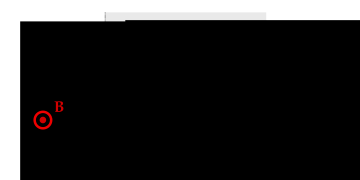
\includegraphics[scale=0.8]{supra}
	\caption{Supraconducteur occupant le demi-espace $x > 0$ baignant dans
	un champ magnétique uniforme $\vecb$ colinéaire à $\ez$.}%
	\label{fig:supra}
\end{figure}

\begin{exocor}[Effet Meissner]
	Dans un matériau supraconducteur, la densité de courant $\mathbf{j}$ 
	vérifie l'équation de London 
\begin{equation*}
	\grad \times \vecj = -\frac{\vecb}{\mu_0 \lambda^2},
\end{equation*} 

où $\mu_0$ est la perméabilité du vide, $\lambda$ une constante dépendant du 
matériau étudié et $\vecb$ le champ magnétique

On se place ici dans un repère carthésien $(0,\ex,\ey,\ez)$. 
Un supraconducteur occupe tout le demi-espace défini par $x > 0$.
À l'extérieur du supraconducteur, le champ est uniforme d'amplitude $B_0$ et 
porté par $\ez$ (voir Fig.~\ref{fig:supra}).
On admettra ici que le champ est continu à la frontière entre le vide et le 
supraconducteur et qu'il ne dépend que de $x$ à l'intérieur de ce dernier.

\begin{enumerate}
	\item Faire une analyse dimensionnelle pour déterminer la dimension de $\lambda$.
	\item Montrer qu'à l'intérieur du supraconducteur, 
	  l'évolution spatiale de l'amplitude du  champ magnétique est donnée par 
		\begin{equation*}
			\dd{^2B}{x^2} - \frac{B}{\lambda^2} = 0.
		\end{equation*}
	On utilisera l'égalité vectorielle suivante, vérifiée pour tout 
	vecteur $\vecb$,
	\begin{equation*} 
		\rot(\rot \vecb) = \gradient(\div\vecb) - \laplacien \vecb,
	\end{equation*}
	où $\laplacien$ correspond à l'opérateur laplacien vectoriel.
	\item La solution générale à cette équation différentielle est de la forme 
\begin{equation}
	B(x) = C \exp(x/\lambda) + D \exp(-x/\lambda),
\end{equation}

où $C$ et $D$ sont deux constantes réelles.
Déterminer l'expression de $C$ et $D$.

\item Pour l'aluminium, $\lambda = 16$\,nm, déterminer le rapport $B(x)/B_0$ pour $x = \lambda,\ 10\lambda,\ 100\lambda$. Proposer alors une interprétation de $\lambda$.
\end{enumerate}

L'impossibilité du champ magnétique externe à pénétrer dans le supraconducteur n'est pas anodine.
Elle induit une force de pression qui s'exerce sur le supraconducteur et peut permettre notamment de faire léviter l'aimant à l'origine de ce champ.. 
Pour en apprendre plus sur les supraconducteurs et leurs propriétés, 
vous pouvez notamment aller voir 
\href{https://www.youtube.com/watch?v=5SF98Ph8hSU}{la vidéo}
\footnote{https://www.youtube.com/watch?v=5SF98Ph8hSU} que 
le Commissariat à l'Énergie Atomique et aux Énergies Alternatives (CEA) a réalisée 
sur le sujet.
\end{exocor}

\begin{exocor}[Champ créé par un câble coaxial]
	On considère un câble coaxial (câble de sortie d'un générateur basse fréquence)
	constitué d'un cylindre métallique central plein de rayon $R_1$ et d'une 
	couche cylindrique de rayon interne $R_2$ et de rayon externe $R_3$. 
	Entre $R_1$ et $R_2$ se trouve une matière isolante assimilable à du vide d'un 
	point de vue électromagnétique. 
	
	On se place dans un repère cylindrique 
	$(O, \er, \etheta, \ez)$. Un point $M$ de l'espace es donc repérér par 
	ses coordonnées $(r, \theta, z)$. Le câble d'axe $(Oz)$ est considéré
	comme infiniment long. La partie conductrice centrale est parcourue 
	par un courant uniforme d'intensité $I$ tandis que la partie périphérique
	est parcourue par un courant uniforme d'intensité $-I$.

	\begin{enumerate}
		\item Réaliser un schéma du système.
		\item Montrer que le champ magnétique $\vecb$ au point $M$ s'écrit
		\begin{equation*}
			\vecb(M) = B(r) \vec{u},
		\end{equation*}
		où $\vec{u}$ est un vecteur à préciser.
		\item Quelle est la valeur du champ magnétique $\vecb$ au point $M$
		  si $r > R_3$ ? Quel est l'avantage d'un câble coaxial par rapport
		  à un simple fil ?
		\item Exprimer les vecteurs densités de courant $\vecj_c$ et 
		  $\vecj_p$ respectivement du conducteur central et du conducteur 
		  périphérique.
		\item Déterminer l'expression du champ magnétique $\vecb$ pour
		  un point $M$ à l'intérieur du câble.
	\end{enumerate}
\end{exocor}
\newpage

